%!TEX root = ../main.tex
\mikkel{An introductiontion needs to be here!}
The on-vehicle network generally have two types of nodes, a generic sensor node and the wifi node.
This section will seek to design and implement software that adheres to the requirements listed earlier.
All nodes in the system needs to:
\begin{itemize}
\item Get data from CAN network.
\item Send data using a CAN controller.
\end{itemize}
As described earlier these responsibilities are implemented in the bare-metal CAN program described in section \ref{sec:methods_to_implement_can} therefore these responsibilities will be omitted from the coming sections .

\subsection{Sensor Node}
\label{sec:sensor_node}
The requirements state that it should be simple to add new sensor nodes to the system. 
To realize this the node software should be designed to be modular.
It should be easily identified what software and what interface a developer of a new sensor node must adhere to.

An example of a node can be seen in figure \ref{fig:gps_node}.

%The coming sections will explain the design of the node software that will provide the mentioned functionality using the design requirement.

\begin{figure}[!h]
\centering
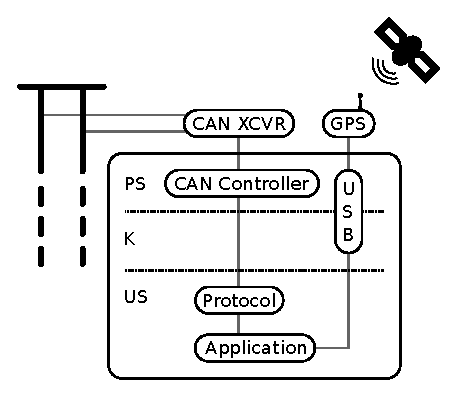
\includegraphics[width=0.5\textwidth]{graphics/analysis_gps.eps}
\caption{GPS node implemented on Zybo board.}
\label{fig:gps_node}
\end{figure}

This specific node has a GPS attached to it connected through a USB interface, but in general it could be any kind of data producing unit connected through any kind of interface.
From the analysis section it is clear that a sensor node has the following responsibilities:

\begin{itemize}
\item Get data from associated sensor.
\item Pack data according to the specified protocol.
\item Construct CAN package
\item React to commands sent to it.
\end{itemize}

Analyzing on the procedure when data goes from a sensor to the CAN program resulted in the block diagram of figure \ref{fig:filter_1}.

\begin{figure}[!h]
    \centering
    \begin{subfigure}{0.45\textwidth}
    \centering
        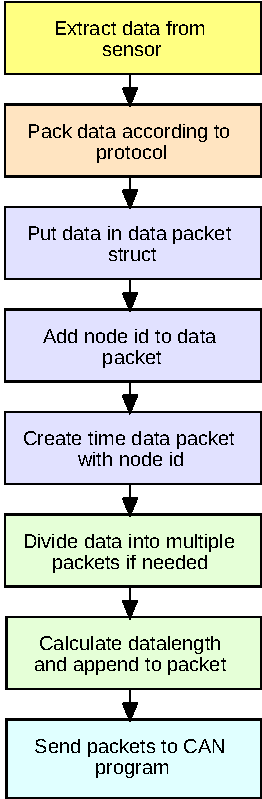
\includegraphics[width=0.60\textwidth]{graphics/FlowChart_Node_Packing}
        \caption{Outgoing data. Data going from a sensor and to the CAN program.}
        \label{fig:filter_1}
    \end{subfigure}
    ~
    \begin{subfigure}{0.45\textwidth}
    \centering
        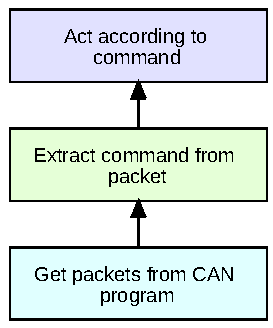
\includegraphics[width=0.60\textwidth]{graphics/FlowChart_Node_Unpacking}
        \caption{Ingoing data. Data going from the CAN program to the node.}
        \label{fig:filter_2}
    \end{subfigure}
        \caption{Block diagram showing handling of outgoing and ingoing data. The boxes are colored according to which class implements the functionality. Yellow is the GPS class, orange is the Packer\_GPS class, blues is the node class, green is the protocol class and blue is the CAN\_link class.}
           \label{fig:filter_fulll}
\end{figure}

To design modular software it needs to be analyzed which blocks are the same for all nodes and which are sensor specific.
The sensor specific tasks are found to be extracting data from sensor and to pack data according to the protocol.
The remaining tasks are the same for all sensor nodes in the system. 
The procedure when data is going from the CAN program to the node is shown in figure \ref{fig:filter_2}.
All tasks are found to be generic for all sensor nodes.

\subsubsection*{Class diagram}
Based on the previous analysis a class diagram was developed and can be seen in figure \ref{fig:node_class_diagram}.
Classes to the right of the dashed vertical is sensor specific and should be developed for each specific sensor.
Shown is the classes for a GPS sensor node. 
\mikkel{Fix this so that it matches the figure}
In a generic sensor node the GPS class would be a sensor class and the Packer\_GPS class would be a Packer\_Sensor.
For the rest of this section the example with a GPS sensor node will be used.
Classes to the left are agnostic to all data they receive going from the sensor and to the CAN network.
They are generic classes and should be reused when developing new nodes.

\begin{figure}[!h]
\centering
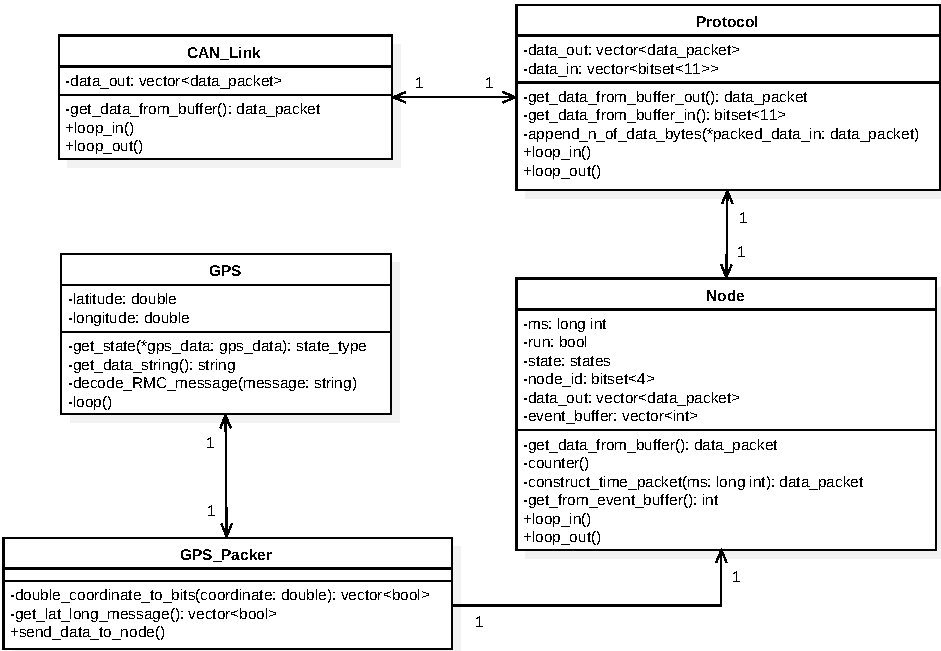
\includegraphics[width=1\textwidth]{graphics/ClassDiagram_NodeSimple}
\caption{Class diagram showing node software.}
\label{fig:node_class_diagram}
\end{figure}

A struct containing all fields of a data packet in boolean data types is defined in listing \ref{code:data_packet}.  

\begin{lstlisting}[caption=Struct for data packet.,label=code:data_packet]
struct data_packet {
  std::bitset<1> nw_msg;
  std::bitset<4> node_id;
  std::bitset<4> dlc;
  std::bitset<6> messagetype;
  std::vector<bool> data; 
(*@\makebox[\linewidth][c]{$\smash{\vdots}$}@*)
};
\end{lstlisting}
It will be passed between the classes and they will each add their own information. 

The classes and their tasks from Code~\ref{code:data_packet} will be explained here.

~\\ \par \textbf{GPS class} ~ \\
The GPS class needs to extract data from a connected GPS unit and update its own variables with that data.
The specific GPS unit used in this project has a USB interface and uses the NMEA protocol to format data.
\mikkel{We are cheating... Explain!}

~\\ \par \textbf{Packer\_GPS class} ~ \\
The Packer\_GPS class is also sensor specific and is the link between the sensor and the data agnostic node.
It is hard-coded with the message types that the sensor is allowed to send onto the network.
It has the responsibility to pack data according to the developed protocol.
Data in the form of a vector of booleans are then put into the \texttt{data\_packet} struct and passed to the node class.
The reason for making a separate class for the packer and not putting the functionality into the GPS class is that if the specification of the protocol or message types change, only this class needs to be modified.

~\\ \par \textbf{Node class} ~ \\
The Node class gets \texttt{data\_packets} from the Packer class and will then prepend its node ID to it.
It needs to create a timestamp \texttt{data\_packet} each time data is to be sent.
In order to create the time message the class needs to keep track of milliseconds since receiving the synchronize message.
The class receives start, stop or synchronize events from the protocol class and reacts to those accordingly.

~\\ \par \textbf{Protocol class} ~ \\
The protocol class receives \texttt{data\_packets} from the node class. 
If it receives \texttt{data\_packets} where there are more than eight data bytes it needs to create additional \texttt{data\_packets} and distribute data to them. 
The additional \texttt{data\_packets} must have the same node id and message types, but the start of frame, sof, bit should be set accordingly.
The class also needs to append number of data bytes, \texttt{n\_data\_bytes}, to each \texttt{data\_packet}.
On \texttt{data\_packets} coming from the CAN network the class needs to use the last two bits of the messagetype to decode which command is sent to the node.
\martin{This is provided, that the CAN controller software filters the messages appropriately.}

~\\ \par \textbf{CAN\_link class} ~ \\
The CAN\_link class has the responsibility of transferring and receiving data to and from the CAN program.
As this interface has not yet been implemented this class makes use of the standard input and output. 
Meaning that data from the sensor will be printed in the shell and data to the node should be written to the shell. 

\subsubsection*{Passing data between classes}
Communication between classes is realised by using the producer-consumer pattern.
As the name implies one class produces data and puts this in a queue where another class consumes by taking data out of the queue.
To get the producer and consumer functions to run in parallel they are run in separate threads.
All queues are protected by a mutex to make the software thread-safe.

\subsubsection*{Node class functionality}
The functionalities of the Node class on outgoing data is implemented using a state machine.
It is shown in figure \ref{fig:state_machine}.
\begin{figure}[!h]
\centering
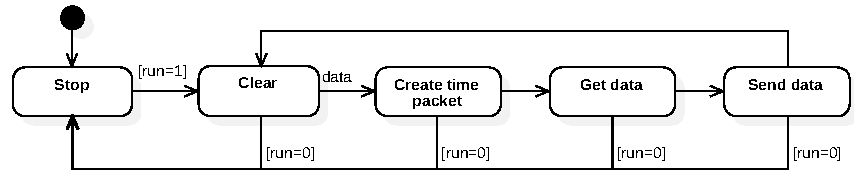
\includegraphics[width=1\textwidth]{graphics/StateDiagram_Node.pdf}
\caption{State machine.....}
\label{fig:state_machine}
\end{figure}
When the variable \texttt{run} is equal to 1, the node should output sensor data.
\texttt{run} is being updated by the thread that handles incoming commands.
It will then go the clear state and clear all variables and wait for data. 
When data is present it will move through the states create time packet, get data and send data. 
If at any point \texttt{run} is set to 0 the state machine will go to the stop state.
In the stop state the input queue of \texttt{data\_packet} will be cleared.

\subsubsection*{Implementing a new Sensor node}
When developing a new node with another sensor the generic classes CAN\_link, Protocol and Node should be used. 
New classes should be developed to extract data from sensor, pack data according to protocol and put the data in a data\_packet.
It is advantageous to implement this functionality into Packer\_Sensor and Sensor classes to keep a similar software design through the nodes.
The interface to the generic Node class is a call to its function \texttt{put\_data\_packet(data\_packet)}.


















\subsection{Wifi Node}
The node with a WiFi connection to the stationary computer is a special node in the system.
There should be only one and it should collect all CAN messages, log them and transfer then using WiFi.
The WiFi node can be seen in figure \ref{fig:wifi_node}.

\begin{figure}[!h]
\centering
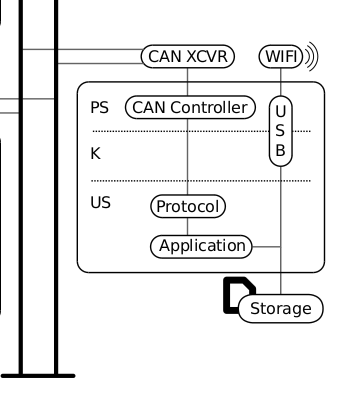
\includegraphics[width=0.4\textwidth]{graphics/wifi_node}
\caption{Figure should be made correctly.}
\label{fig:wifi_node}
\end{figure}

From the analysis it is clear that the WiFi node has the following responsibilities:

\begin{itemize}
\item Log all data to SD card.
\item Transmit and receive data through WiFi.
\item Pack data according to protocol
\item Send log file through WiFi.
\item Timestamp management
\item Merge multi frame packets
\end{itemize}
\mikkel{Is multi frame packets what we mean?}

It is found that the responsibilities can be grouped into normal operation mode and sending log file mode.
This should be implemented as a state machine as shown in figure \ref{fig:StateDiagram_NodeWiFiStates}.
In normal operation mode the WiFi node should handle data coming from the CAN network and the data coming from the WiFi connection.
If it receives a \texttt{send\_log} command from the stationary computer it should go into the sending log mode and stay there until the log file has been sent.

\begin{figure}[!h]
\centering
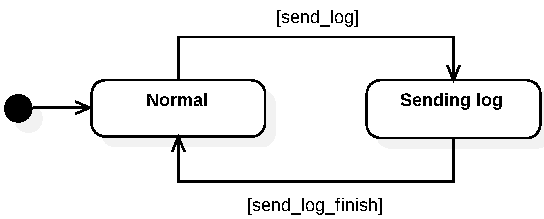
\includegraphics[width=0.5\textwidth]{graphics/StateDiagram_NodeWiFiStates}
\caption{State machine in WiFi node software.}
\label{fig:StateDiagram_NodeWiFiStates}
\end{figure}

In normal operation mode it should handle all incoming data from the WiFi connection as shown in figure \ref{fig:FlowChart_NodeWiFiCmd}.
As it can be seen the WiFi node will only send frames to the CAN network when it receives commands to do so from the stationary computer.
\begin{figure}[!h]
\centering
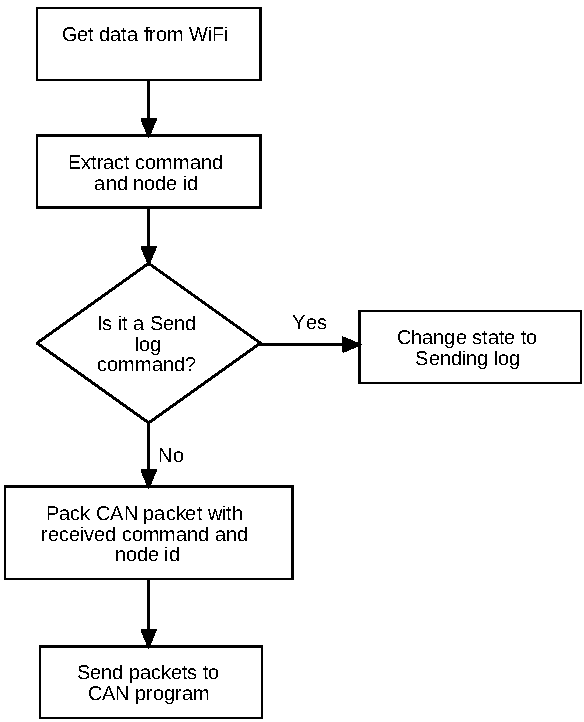
\includegraphics[width=0.5\textwidth]{graphics/FlowChart_NodeWiFiCmd}
\caption{B}
\label{fig:FlowChart_NodeWiFiCmd}
\end{figure}

\begin{figure}[!h]
\centering
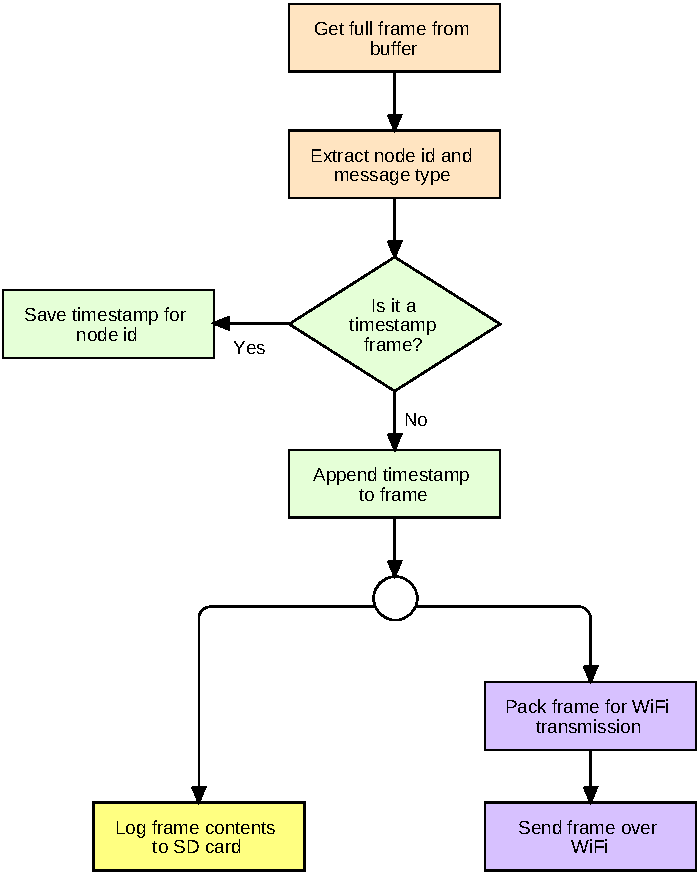
\includegraphics[width=0.6\textwidth]{graphics/FlowChart_CANFrameProcess}
\caption{Cxxx}
\label{fig:FlowChart_CANFrameProcess}
\end{figure}


\begin{figure}[!h]
\centering
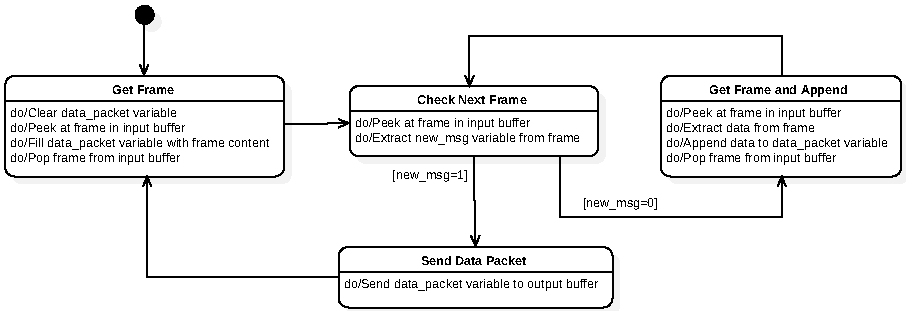
\includegraphics[width=1\textwidth]{graphics/StateDiagram_ConcatMsgProcess}
\caption{cccc}
\label{fig:StateDiagram_ConcatMsgProcess}
\end{figure}



\begin{figure}[!h]
    \centering
    \begin{subfigure}{0.42\textwidth}
    \centering
        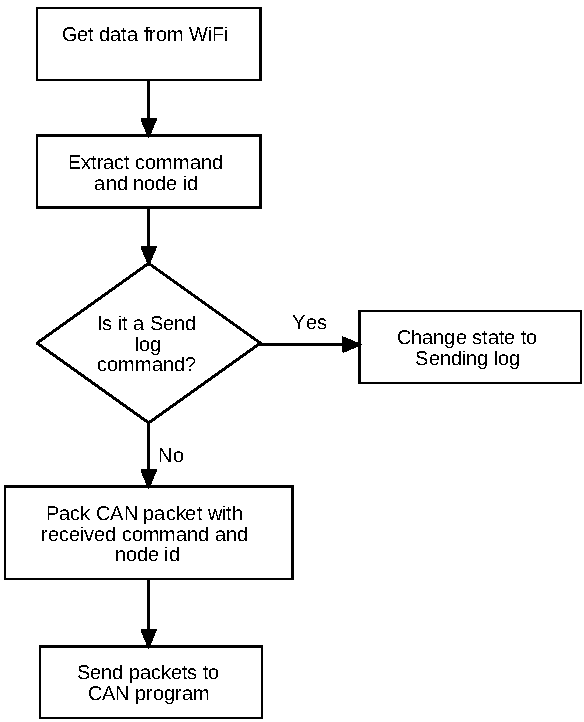
\includegraphics[width=1\textwidth]{graphics/FlowChart_NodeWiFiCmd}
        \caption{Outgoing data. Data going from a sensor and to the CAN program.}
        \label{fig:filter_1}
    \end{subfigure}
    ~
    \begin{subfigure}{0.52\textwidth}
    \centering
        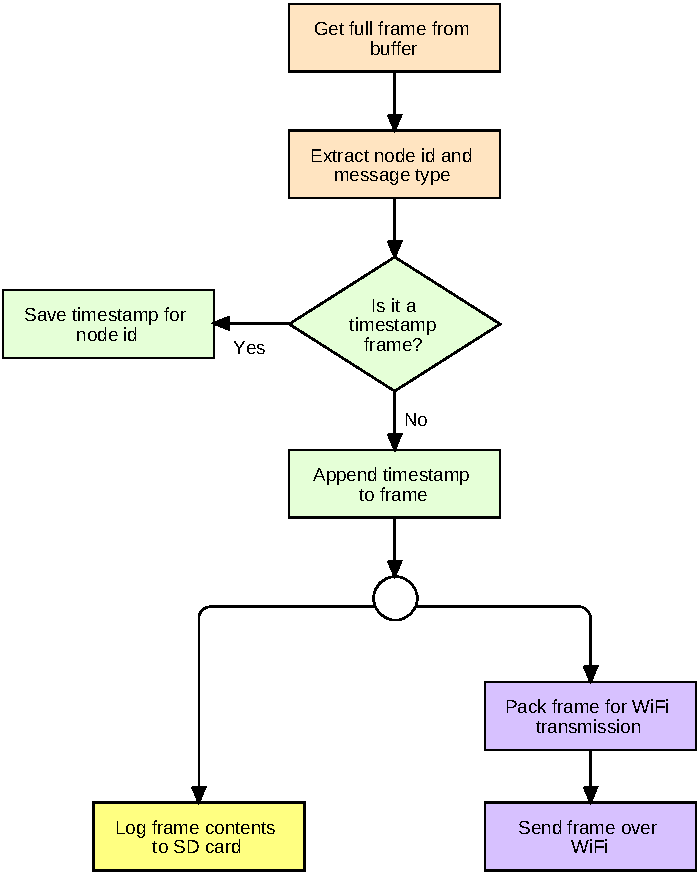
\includegraphics[width=1\textwidth]{graphics/FlowChart_CANFrameProcess}
        \caption{Ingoing data. Data going from the CAN program to the node.}
        \label{fig:filter_2}
    \end{subfigure}
        \caption{Block diagram showing handling of outgoing and ingoing data. The boxes are colored according to which class implements the functionality. Yellow is the GPS class, orange is the Packer\_GPS class, blues is the node class, green is the protocol class and blue is the CAN\_link class.}
           \label{fig:filter_fulll}
\end{figure}
